\section{Mediciones, tests y experimentos}
\subsection{Tests de correctitud}
Para los ejercicios 1 y 2 se realizaron ademas de las mediciones, tests de correctitud, se detalla a continuaci\'on como fueron implementados:
\begin{itemize}
	\item \textbf{Ejercicio 1:} Se program\'o un algoritmo mas simple en O($n^2$) que asumimos como v\'alido y se compararon todas las salidas de este algoritmo versus el algoritmo mas eficiente(y por lo tanto mas complejo). 
	\item \textbf{Ejercicio 2:} Se constat\'o que todas las salidas, estuvieran ordenadas seg\'un el criterio indicado en la demostraci\'on de correctitud del ejercicio 2.
\end{itemize}

\subsection{Forma de medici\'on}
Con la ayuda de una macro creada especialmente para ser reutilizada en todas las porciones cr\'iticas de c\'odigo que quisieramos medir, las mediciones fueron realizadas con la herramienta $high\_resolution\_clock$ provista por la libreria $chrono$ de $C++$. Dicha macro provee una forma pr\'actica de obtener la cantidad promedio de microsegundos consumidos por el c\'odigo que se desea medir. Se le pasan como par\'ametros el c\'odigo a ejecutar, la cantidad de veces que se repetir\'a el experimento para tomar el promedio y una referencia a la variable en la que se guardar\'a el resultado de la medici\'on. 

\subsection{Porciones cr\'iticas de c\'odigo a medir de los ejercicios}
Los ejercicios se basan en 3 secciones principales:
\begin{enumerate}
	\item Lectura y decodificaci\'on de la entrada estandar.
	\item Procesamiento y transformaci\'on de los datos de entrada para producir la salida
	\item Codificaci\'on de la salida y escritura a salida estandar.
\end{enumerate}

En particular lo que nos interesa medir a nosotros, es unicamente el inciso 2 de la lista anterior, no nos interesa tomar mediciones de entrada-salida, pues esto no es parte intr\'inseca del algoritmo. Tanto para los ejercicios 1 y 2 se realizaron 100 repeticiones para obtener el promedio de las mediciones y licuar posibles valores at\'ipicos. Para el caso del ejercicio 3 este numero de repeticiones se vio disminuido a aproximadamente 10 repeticiones dada la complejidad mas alta del algoritmo.

\subsection{Ejercicio 1}
En este algoritmo, hemos determinado una cota de complejidad temporal asint\'otica te\'orica de O(n.log(n)).(Detalles en la secci\'on complejidad de dicho ejercicio).
La entrada ha sido expresado en n = \#\{ Cantidad de camiones \} y sobre este numero se ha realizado la medici\'on. Las mediciones de los experimentos que hemos realizado se condicen con esta cota te\'orica, a continuaci\'on se explicar\'a como fue obtenida esta conclusi\'on.\\

Aqu\'i observamos un gr\'afico de los pares $(x, f(x))$ no demasiado claro respecto a que funcion representa, aunque parece lineal, mas que linear\'itmico, probamos variando la cantidad de elementos pero no obtuvimos mejora. Creemos se debe a que el logaritmo crece muy lentamente, lo cual se confirma mas adelante en el texto con nuevos experimentos.  
\begin{center}
	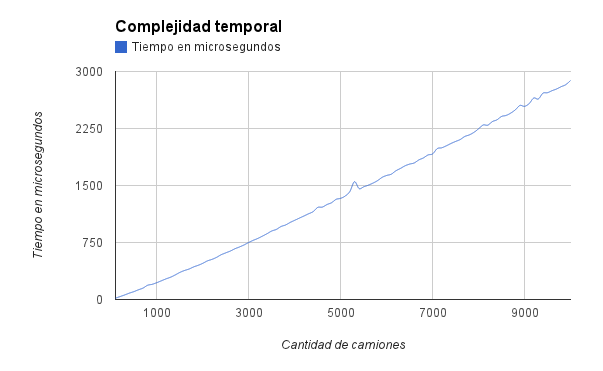
\includegraphics[scale=0.6]{images/ej1_fx.png}
\end{center}

Luego del primer grafico obtenido, decidimos graficar los pares $(x, \frac{f(x)}{x})$ con el objetivo de obtener un gr\'afico consistente con una funcion logaritmica, el resultado es el esperado, se puede observar un comportamiento logar\'itmico en el crecimiento de la funcion graficada. Notemos ademas, la imagen de la funcion resultante, esta acotada en el intervalo $\left[ 0.18 \dots 0.30\right]$, con lo cual, una funcion lineal multiplicada por valores en este intervalo, no se ver\'a alterada en exceso, explicando el grafico original obtenido en la medici\'on.
\begin{center}
	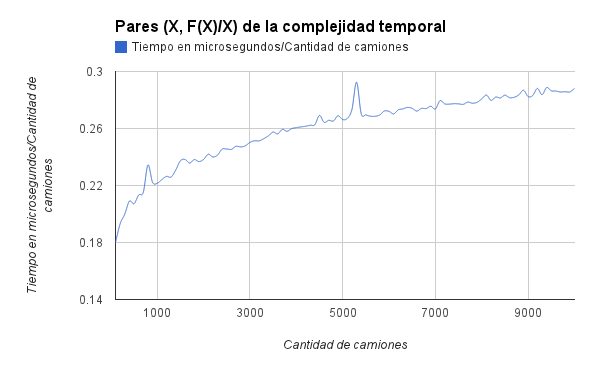
\includegraphics[scale=0.6]{images/ej1_fx_x.png}
	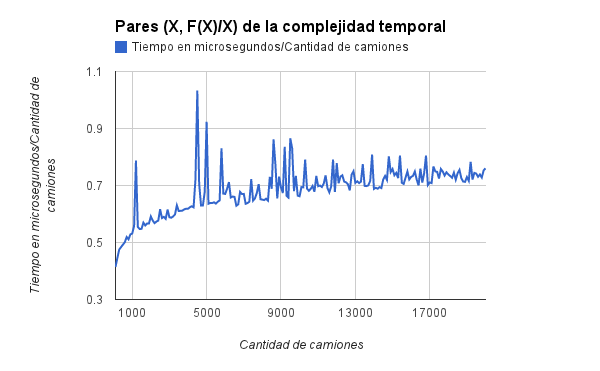
\includegraphics[scale=0.6]{images/ej1_fx_x_bis.png}
\end{center}

Como medida adicional, tambien graficamos los pares $(x, \frac{f(x)}{Log(x)})$ para tener una mayor certeza acerca de la funcion inicial. Podemos observar una funcion que es una escala de la funci\'on original, lo cual tiene sentido, dado el intervalo acotado del logaritmo que acompa\~na la funcion lineal multiplicando en la expresi\'on  \textbf{junto a una constante positiva menor que uno}. Probamos en dos casos, uno con una gran amplitud en en el intervalo de generacion de numeros aleatorios para los dias de la entrada, y otro con una amplitud m\'as limitada, el resultado fue el mismo en todos los gr\'aficos salvo en el logaritmico, lo cual puede explicarse por la busqueda binaria que se realiza sobre el conjunto de tuplas ordenadas (Dia, Cantidad de camiones hasta ese dia), lo cual tiene una complejidad O(k.logk) donde k = \#\{Cantidad de dias distintos en la entrada\}
\begin{center}
	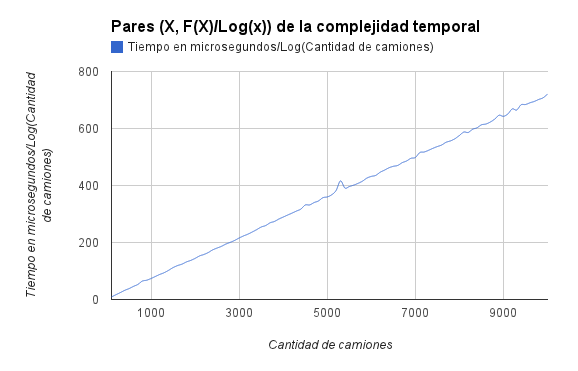
\includegraphics[scale=0.6]{images/ej1_fx_logx.png}
\end{center}

Finalmente graficamos los pares $(x, \frac{f(x)}{x*Log(x)})$ para constatar que se obtendr\'ia una constante, vamos que en realidad la funci\'on fluctua, pero dentro de un intervalo muy peque\~no $\left[ 0.07 \dots 0.09\right]$, lo cual consideramos es aceptable para asegurar que es una constante.

\begin{center}
	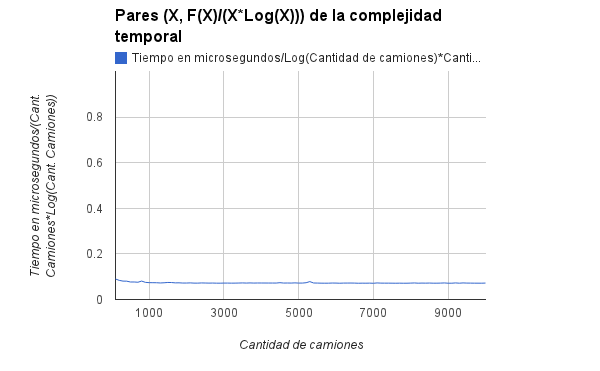
\includegraphics[scale=0.6]{images/ej1_fx_xlogx.png}
\end{center}

Como conclusi\'on podemos asegurar que el algoritmo tiene realmente la complejidad te\'orica esperada.


\subsubsection{Caso Promedio}

Para el caso promedio simplemente probamos varias intancias generadas aleatoriamente

\subsubsection{Mejor Caso}

Luego de analizar nuestro algoritmo consideramos que el mejor caso posible se da cuando el vector de entrada posee todos sus elementos iguales, es decir, todos los camiones llegan el mismo d\'ia. El ordenamiento que realiza nuestro algoritmo al comenzar se llama $introsort$, de la librer\'ia de C++, que comienza con quicksort, cambia a heapsort cuando la cantidad de llamadas recursivas excede $2*log_2(n)$. En un array de elementos iguales, la perfomance del Quicksort va a ser $(n log n)$, ya que el pivote que va a tomar en cada una de las iteraciones va a ser exactamente la mediana, causando que los dos \'indices del ciclo se unan exactamente en el medio, dividiendo los dos subproblemas en exactamente la mitad de tamano.

\vspace{2mm}

Vemos dr\'asticamente una mejora en la perfomance en la segunda parte del algoritmo. En la funci\'on que agrupa y acumula, al ser todos los elementos id\'enticos, el vector tablaDiaCantidad va a tener un solo elemento, la tupla $<unico \: elemento, longitud\_entrada>$. Por lo cual el ciclo principal del algoritmo va a realizar s\'olo una iteraci\'on hasta encontrar el intervalo \'optimo, que es el \'unico posible, el que comienza con el \'unico d\'ia en que llegan todos los camiones.

\subsubsection{Peor Caso}

No pudimos encontrar la implementaci\'on del introsort, por lo cual no sabemos qu\'e' m\'etodo utiliza para tomar el pivote. Por lo cual no sabemos cu\'al es el peor caso de este ordenamiento. De todas formas al tener complejidad $O(nlogn)$ para cualquier caso posible, la disposici\'on de los enteros del vector de entrada no influye demasiado. Busquemos peor caso de la segunda parte del algoritmo. Acto seguido del ordenamiento nuestro algoritmo recorre 1 vez el vector de entrada agrupando repetidos y acumulando. Esto es siempre linea, va a iterar una vez por cada elemento siempre, pero el peor caso posible del algoritmo debe tener todos los d\'ias de entrada distintos, as\'i esta reducci\'on efectivamente no reduce nada, y el vector resultante tablaDiaCantidad sigue siendo de longitud $n$.



\vspace{2mm}

El ciclo principal de nuestro algoritmo recorre una vez el vector tablaDiaCantidad. Por cada iteraci\'on realiza una b\'usqueda binaria. El peor caso de la b\'usqueda binaria es cuando el n\'umero a buscar no se encuentra en el arreglo. Con lo cual, para cada iteraci\'on, si para cada d\'ia $inicio$, el d\'ia $inicio + D - 1$ no se encuentra en el arreglo nos aseguraremos de que la b\'usqueda realiza la mayor cantidad de pasos posibles. Adem\'as, si $D=1$, el d\'ia a buscar queda en el extremo izquierdo del intervalo a buscar, y si $D=n$, queda siempre en el extremo derecho, lo cual tambi\'en son los peores casos de la b\'usqueda binaria. Por lo cual vamos a testear dos tipos de casos. En ambos la la distribuci\'on de d\'ias es uniforme, en el primer tipo $D=1$ y para cada d\'ia $inicio$, el d\'ia $inicio + D - 1$ nunca est\'a. En el segundo tipo de caso $D$ va a ser igual a $n$, con lo cual $inicio + D - 1$ siempre va a caer afuera del arreglo.

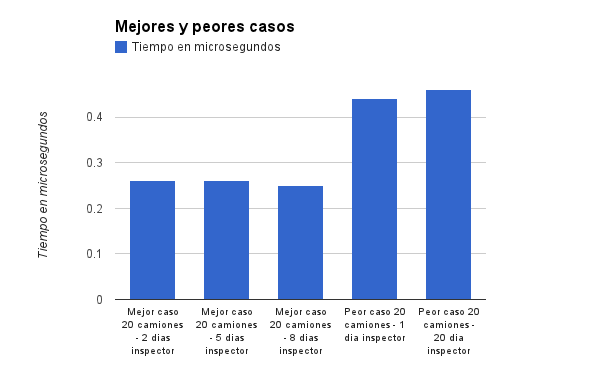
\includegraphics[scale=0.750]{images/ej1_mejor_peor.png}

\subsection{Ejercicio 2}
Para el algoritmo del ejercicio 2, tambien se observ\'o una complejidad asint\'otica te\'orica O(n.log(n)). La medici\'on de la entrada fue sobre n = \#\{ Cantidad de joyas pendientes \}. Se realiz\'o un razonamiento an\'alogo al ejercicio anterior para constatar con seguridad que se condicen las mediciones emp\'iricas con la cota te\'orica. A continuaci\'on se indican las mediciones, nuevamente graficamos la funcion original obtenida de las mediciones, dividimos sucesivamente por n, logn y finalmente nlogn obteniendo nuevamente las mismas conclusiones que en el ejercicio anterior, aunque esta vez, la funci\'on logaritmica obtenida en los pares $(x, \frac{f(x)}{x})$, es mas irregular y la funcion constante esta mas acotada dentro de un intervalo mas ajustado. Finalmente este ejercicio tambien posee una complejidad que condice con la hallada teoricamente.\\
Podemos indicar adem\'as que el peor y mejor caso de este algoritmo depende fuertemente de la implementaci\'on del algoritmo de ordenamiento de la librer\'ia de $C++$ ya que el resto del algoritmo es lineal y muy simple como para interferir con casos particulares.

\begin{center}
	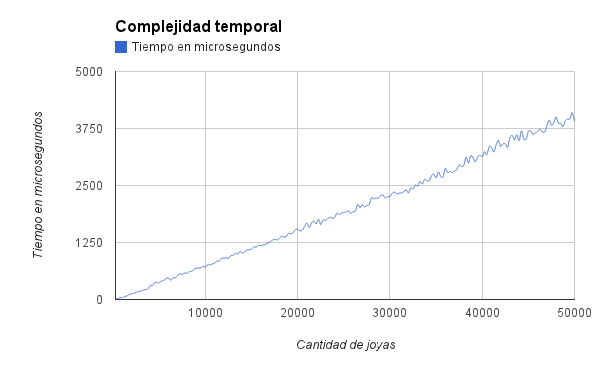
\includegraphics[scale=0.60]{images/ej2_fx.png}
	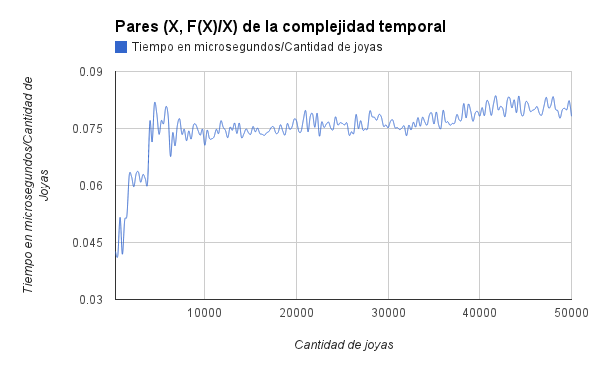
\includegraphics[scale=0.60]{images/ej2_fx_x.png}
\end{center}

\begin{center}
	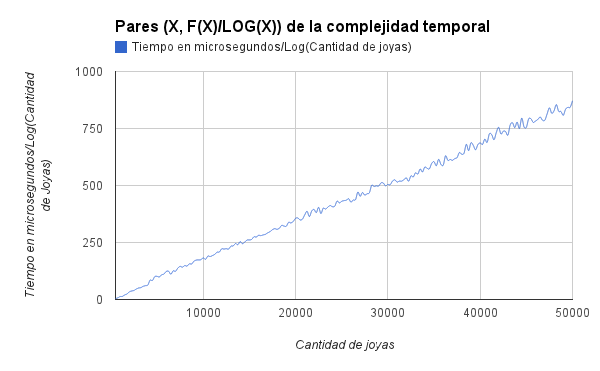
\includegraphics[scale=0.60]{images/ej2_fx_logx.png}
	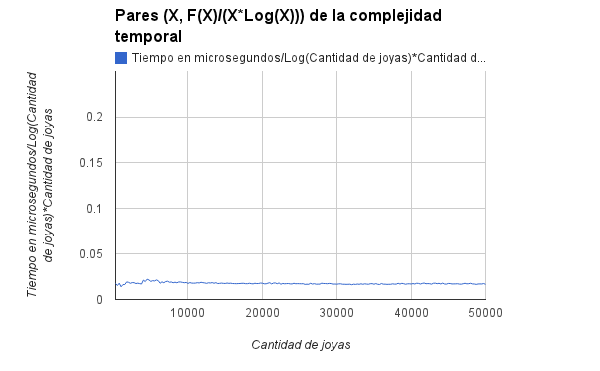
\includegraphics[scale=0.60]{images/ej2_fx_xlogx.png}
\end{center}

\subsection{Ejercicio 3} \label{mediciones_3}

Con el caso del ejercicio 3, como la complejidad es muy grande, no se pudieron realizar muchos casos de prueba con valores grandes de la entrada.

Se plante\'o como mejor caso el caso en que todas las fichas est\'en ordenadas de la forma que deben ser colocadas (o bien que todas las fichas tengan todos los lados del mismo color), por lo que encuentra el m\'aximo en $n*m$ como se explic\'o en la secci\'on \ref{ej_3:cota}, y se teste\'o dicho caso.

Tambi\'en se plante\'o como peor caso el que la poda no se realize y que pruebe la mayor cantidad de combinaciones posibles. Para lograr la mayor cantidad de combinaciones v\'alidas todas las fichas deben poder colocarse de todas las maneras posibles entre s\'i, pero si \'esto ocurriese, ser\'ia el mejor caso porque encuentra el m\'aximo valor posible de fichas a colocar en la primera iteraci\'on, entonces para minimizar la cantidad de combinaciones que se descartan, se puede poner que s\'olo una ficha no se pueda poner junto con las otras,
por ejemplo, que todas las fichas sean totalmente verdes menos 1 que sea roja. en \'este caso el primer tablero que encuentre tendr\'a $n*m - 1$ fichas colocadas, por la poda, todas las demas combinaciones que tengan 1 o m\'as casillero vac\'ios ser\'an descartadas, por lo que tenemos en total $(n*m-1)!$ combinaciones a probar.

Gr\'afico con el taman\~no de la entrada siendo la cantidad de casilleros del tablero, y el tiempo en microsegundos, se separ\'o en 2 gr\'aficos para que se aprecien los valores con entrada m\'as chica:
\begin{center}
	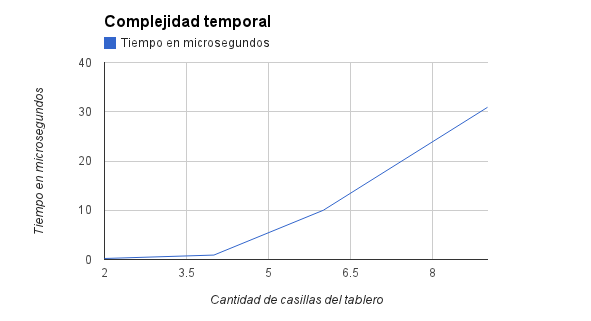
\includegraphics[scale=0.70]{images/ej3_tiempo1.png}
\end{center}
\begin{center}
	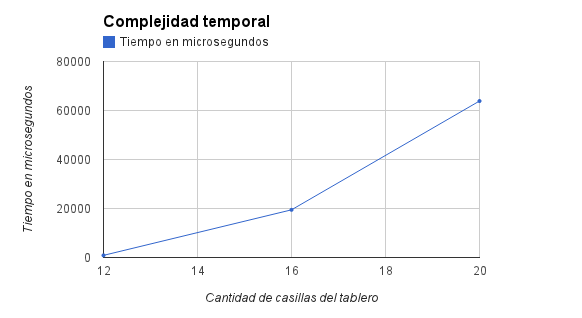
\includegraphics[scale=0.70]{images/ej3_tiempo2.png}
\end{center}

Luego se midieron los peores y mejores caso para tableros de 3x3 y 4x4 casilleros, para el peor caso de 4x4 cortamos la ejecuci\'on porque tom\'o mas de una hora y nos parecio demasiado.
\begin{center}
	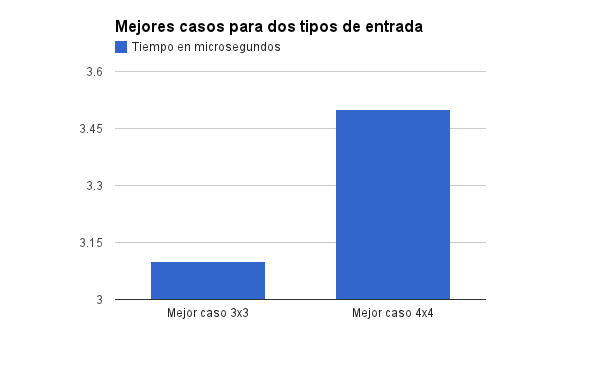
\includegraphics[scale=0.70]{images/ej3_mejor_caso.png}
	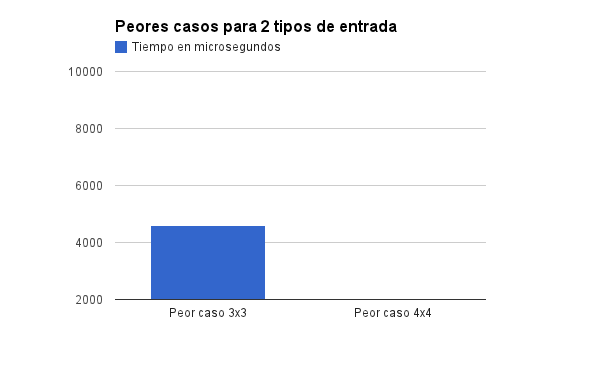
\includegraphics[scale=0.70]{images/ej3_peor_caso.png}
\end{center}

Al no poder correr una cantidad muy variada de casos con diferentes tama\~nos de la entrada, no podemos asegurar mucho sobre los gr\'aficos, de todas formas al tiempo que tard\'o cada caso, se lo dividi\'o por $(n*m)^2$ y por $(n*m)!$ para ver si la curva se llevaba a una recta
\begin{center}
	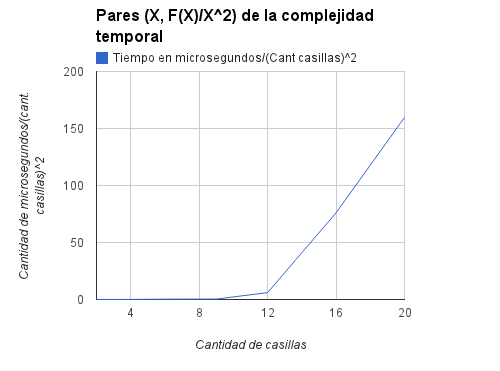
\includegraphics[scale=0.70]{images/ej3_cuadratica.png}
	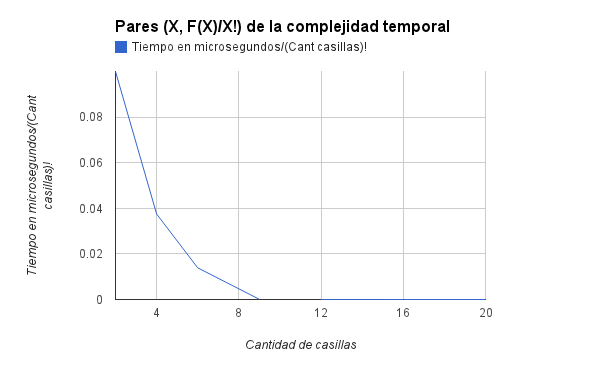
\includegraphics[scale=0.70]{images/ej3_factorial.png}
\end{center}

Como se ve, al dividir por la cuadr\'atica al menos para los primeros valores la curva a\'un est\'a creciendo, con lo cual esta no es una cota v\'alida.Asimismo cuando se divide por el factorial la curva decrece y tiende a cero, y dado que la funcion original de complejidad es creciente, podemos asegurar que la complejidad est\'a acotada por debajo por O($(n*m)^2$) y por encima por O((n*m)!) .

